\documentclass{article}

\usepackage[spanish]{babel}
\usepackage[utf8]{inputenc}
\usepackage[T1]{fontenc}
\usepackage{graphicx}
\usepackage{wrapfig}
\usepackage{pdfpages}
\usepackage{hyperref}
\usepackage{courier}
\usepackage{longtable}
\usepackage{listings}
\usepackage{minted}
\usepackage{xcolor}
\usepackage{blindtext}
\usepackage{scrextend}
\usepackage[document]{ragged2e}
\usepackage{multicol}
\usepackage{booktabs}
\usepackage{amsmath}
 % % % % % % % %

\usemintedstyle{pastie}

\usepackage{array}
\newcolumntype{L}[1]{>{\raggedright\let\newline\\\arraybackslash\hspace{0pt}}m{#1}}
\newcolumntype{C}[1]{>{\centering\let\newline\\\arraybackslash\hspace{0pt}}m{#1}}
\newcolumntype{R}[1]{>{\raggedleft\let\newline\\\arraybackslash\hspace{0pt}}m{#1}}

%Custom commands
\newcommand\myeq{\mathrel{\overset{\makebox[0pt]{\mbox{\normalfont\tiny\sffamily 24 Ceros}}}{00\dots00}}}

\usepackage{anysize}
\marginsize{2.54cm}{2.54cm}{2.54cm}{2.54cm}

\usepackage{setspace}
\onehalfspacing
%\doublespacing

\setlength{\columnsep}{1cm}

%En caso de que LaTeX separe las palabras con - de manera incorrecta, usar
%\hyphenation{deci-sión,e-xa-men, otras palabras....}

\setlength{\columnseprule}{2pt}
\def\columnseprulecolor{\color{black}}


% Aqui comienza el documento como tal!!
\begin{document}

\flushleft
\setlength{\parindent}{20pt}

\justify
%%CUERPO PRINCIPAl%%%%%%%%%%%%%%%%%%%%%%%%%%%%%%%%%%%%%%%%%%%
\centerline{\huge Tarea 1 \textbf{Calculo Computacional}}
\centerline{Victor Tortolero CI:24.569.609}  % Pon tu nombre y Cedula!
\vspace{0.1cm}
\hrule

%% Respuesta 1 %%%%%%%%%%%%%%%%%%	
\section*{Respuesta 1}
Tenemos que $\frac{A + 3}{13}$, como $A = 9$, tendríamos $\frac{9 + 3}{13} = \frac{12}{13}$.
Ahora procedemos a convertir a binario. \newline
\begin{multicols}{2}
	$\frac{12}{13} \times 2 = \frac{24}{13}$, $b_{0} = 1$ \newline
	$\frac{11}{13} \times 2 = \frac{22}{13}$, $b_{1} = 1$ \newline
	$\frac{9}{13} \times 2 = \frac{18}{13}$, $b_{2} = 1$ \newline
	$\frac{5}{13} \times 2 = \frac{10}{13}$, $b_{3} = 0$ \newline
	$\frac{10}{13} \times 2 = \frac{20}{13}$, $b_{4} = 1$ \newline
	$\frac{7}{13} \times 2 = \frac{14}{13}$, $b_{5} = 1$ \newline
	$\frac{1}{13} \times 2 = \frac{2}{13}$, $b_{6} = 0$ \newline
	$\frac{2}{13} \times 2 = \frac{4}{13}$, $b_{7} = 0$ \newline
	$\frac{4}{13} \times 2 = \frac{8}{13}$, $b_{8} = 0$ \newline
	$\frac{8}{13} \times 2 = \frac{16}{13}$, $b_{9} = 1$ \newline
	$\frac{3}{13} \times 2 = \frac{6}{13}$, $b_{10} = 0$ \newline
	$\frac{6}{13} \times 2 = \frac{12}{13}$, $b_{11} = 0$ \newline
\end{multicols}

Por lo tanto tenemos que:
\begin{equation*}
	0.111011000100\overline{111011000100}\textbf{1}\dots
\end{equation*}
Observemos que el numero que vendria luego del bit 24 seria un 1. Entonces a la hora de redondear se suma 1.
Por lo tanto, tenemos que $Fl(\frac{12}{13})_{Truncado} = 0.111011000100111011000100$, 
y que $Fl(\frac{12}{13})_{Redondeado} = 0.111011000100111011000101$.
\begin{align*}
	\text{\textbf{Por Truncamiento tenemos que:}} \\
	E_{A} = |x - Fl(x)_{Truncado}| & = 0, \underbrace{000\dots000}_\text{24 Ceros}111011000100\dots \\
	& = 0,\underbrace{111011000100111011000100}_\text{Esto es $\frac{12}{13}$}\dots \times 2^{-24} \\
	& = \frac{12}{13} \times 2^{-24} \approx 5,50196 \times 10^{-8} \\
	E_{R} = \frac{E_{A}}{|x|} & = \frac{\frac{12}{13} \times 2^{-24}}{\frac{12}{13}} \\
	& = 2^{-24} \approx 5,96046 \times 10^{-8}
\end{align*}

\begin{align*}
\text{\textbf{Por Redondeo tenemos que:}} \\
E_{A} = |x - Fl(x)_{Redondeado}| & = |x - (Fl(x)_{Truncado} + 1 \times 2^{-24})| \\
& = |x - Fl(x)_{Truncado} - 1 \times 2^{-24}| \\
& = |\frac{12}{13} \times 2^{-24} - 1 \times 2^{-24}|  \\
& = |\frac{12}{13} - 1| \times 2^{-24} \\
& = \frac{1}{13} \times 2^{-24} \approx 4,584 \times 10^{-9} \\
E_{R} = \frac{E_{A}}{|x|} & = \frac{\frac{1}{13} \times 2^{-24}}{\frac{12}{13}} \\
& = \frac{1}{12} \times 2^{-24} \approx 4,9670 \times 10^{-9}
\end{align*}
%%%%%%%%%%%%%%%%%%%%%%%%%%%%%%%%%%%%%%	


%% Respuesta 2 %%%%%%%%%%%%%%%%%%%%%%
\hrule
\section*{Respuesta 2}
Tenemos $245696,09_{10}$, procedemos a convertirlo a binario:

\begin{itemize}
	\item \textbf{Parte Entera}:
	\begin{multicols}{2}
		$\frac{245696}{2} = 122848$, $b_{17} = 0$ \newline
		$\frac{122848}{2} = 61424$, $b_{16} = 0$ \newline
		$\frac{61424}{2} = 30712$, $b_{15} = 0$ \newline
		$\frac{30712}{2} = 15356$, $b_{14} = 0$ \newline
		$\frac{15356}{2} = 7678$, $b_{13} = 0$ \newline
		$\frac{7678}{2} = 3839$, $b_{12} = 0$ \newline
		$\frac{3839}{2} = 1919$, $b_{11} = 1$ \newline
		$\frac{1919}{2} = 959$, $b_{10} = 1$ \newline
		$\frac{959}{2} = 479$, $b_{09} = 1$ \newline
		$\frac{479}{2} = 239$, $b_{08} = 1$ \newline
		$\frac{239}{2} = 119$, $b_{07} = 1$ \newline
		$\frac{119}{2} = 59$, $b_{06} = 1$ \newline
		$\frac{59}{2} = 29$, $b_{05} = 1$ \newline
		$\frac{29}{2} = 14$, $b_{04} = 1$ \newline
		$\frac{14}{2} = 7$, $b_{03} = 0$ \newline
		$\frac{7}{2} = 7$, $b_{02} = 1$ \newline
		$\frac{3}{2} = 1$, $b_{01} = 1$ \newline
		$\frac{1}{2} = 0$, $b_{00} = 1$ \newline
	\end{multicols}
	Por lo tanto tenemos que $245696_{10} = 111011111111000000_{2}$.
	
	\item \textbf{Parte Decimal}:
	\begin{multicols}{2}
		$\frac{9}{100} \times 2 = \frac{18}{100}$, $b_{0} = 0$ \newline
		$\frac{18}{100} \times 2 = \frac{36}{100}$, $b_{1} = 0$ \newline
		$\frac{36}{100} \times 2 = \frac{27}{100}$, $b_{2} = 0$ \newline
		$\frac{72}{100} \times 2 = \frac{144}{100}$, $b_{3} = 1$ \newline
		$\frac{44}{100} \times 2 = \frac{88}{100}$, $b_{4} = 0$ \newline
		$\frac{88}{100} \times 2 = \frac{176}{100}$, $b_{5} = 1$ \newline
		$\frac{76}{100} \times 2 = \frac{152}{100}$, $b_{6} = 1$ \newline
		$\frac{52}{100} \times 2 = \frac{104}{100}$, $b_{7} = 1$ \newline
	\end{multicols}
	Por lo tanto tenemos que $0,09_{10} = 00010111$.
\end{itemize}
{\noindent
	Entonces se tiene que $245696,09_{10} \approx \overbrace{111011111111000000,000101}^{24 bits}11_{2}$. \newline

\noindent	
	Si usamos \textbf{redondeo:} \newline
	$\boldsymbol{Fl(245696,09)_{Redondeado} = 0,111011111111000000000110 \times 2^{18}}$
	\newline

\noindent	
	Si representamos este numero de vuelta en \textbf{decimal:} \newline
	$\boldsymbol{111011111111000000,000110_{2} = 245696,09375_{10}}$. \newline
	

\noindent	
	\textbf{Error absoluto y relativo}:
	\begin{align*}
	E_{A} = |x - Fl(x)_{Redondeado}| & = |245696,09 - 245696,09375| \\
	& = 3.75 \times 10^{-3} \\
	E_{R} = \frac{E_{A}}{|x|} & = \frac{3,75 \times 10^{-3}}{245696,09} \approx -1.526275815 \times 10^{-8} \\
	\end{align*}
}	
%%%%%%%%%%%%%%%%%%%%%%%%%%%%%%%%%%%%%%


%% Respuesta 3 %%%%%%%%%%%%%%%%%%%%%%
\hrule
\section*{Respuesta 3}



Después de correr el programa, se obtuvieron los siguientes datos
\begin{itemize}
	\item \textbf{Para simple precisión}:
	$\epsilon = 0.0000001192092895507812500000000000$ \newline
	\begin{longtable}{|c||c|c|}
		\hline
		Iteracion & t & $\epsilon$ \\ \hline \hline
		1 & 1.500000000000000000000000 & 0.5000000000000000000000000000000000 \\  \hline
		2 & 1.250000000000000000000000 & 0.2500000000000000000000000000000000 \\  \hline
		3 & 1.125000000000000000000000 & 0.1250000000000000000000000000000000 \\  \hline
		4 & 1.062500000000000000000000 & 0.0625000000000000000000000000000000 \\  \hline
		5 & 1.031250000000000000000000 & 0.0312500000000000000000000000000000 \\  \hline
		6 & 1.015625000000000000000000 & 0.0156250000000000000000000000000000 \\  \hline
		7 & 1.007812500000000000000000 & 0.0078125000000000000000000000000000 \\  \hline
		8 & 1.003906250000000000000000 & 0.0039062500000000000000000000000000 \\  \hline
		9 & 1.001953125000000000000000 & 0.0019531250000000000000000000000000 \\  \hline
		10 & 1.000976562500000000000000 & 0.0009765625000000000000000000000000 \\  \hline
		11 & 1.000488281250000000000000 & 0.0004882812500000000000000000000000 \\  \hline
		12 & 1.000244140625000000000000 & 0.0002441406250000000000000000000000 \\  \hline
		13 & 1.000122070312500000000000 & 0.0001220703125000000000000000000000 \\  \hline
		14 & 1.000061035156250000000000 & 0.0000610351562500000000000000000000 \\  \hline
		15 & 1.000030517578125000000000 & 0.0000305175781250000000000000000000 \\  \hline
		16 & 1.000015258789062500000000 & 0.0000152587890625000000000000000000 \\  \hline
		17 & 1.000007629394531200000000 & 0.0000076293945312500000000000000000 \\  \hline
		18 & 1.000003814697265600000000 & 0.0000038146972656250000000000000000 \\  \hline
		19 & 1.000001907348632800000000 & 0.0000019073486328125000000000000000 \\  \hline
		20 & 1.000000953674316400000000 & 0.0000009536743164062500000000000000 \\  \hline
		21 & 1.000000476837158200000000 & 0.0000004768371582031250000000000000 \\  \hline
		22 & 1.000000238418579100000000 & 0.0000002384185791015625000000000000 \\  \hline
		23 & 1.000000119209289600000000 & 0.0000001192092895507812500000000000 \\  \hline
		24 & 1.000000000000000000000000 & 0.0000000596046447753906250000000000 \\  \hline
	\end{longtable}
	
	\vspace{0.2cm}
	\item \textbf{Para doble precisión}:
	$\epsilon =  0.0000000000000002220446049250313100$ \newline
	\begin{longtable}{|c||c|c|}
		\hline
		Iteracion & t & $\epsilon$ \\ \hline \hline
		1 & 1.500000000000000000000000 & 0.500000000000000000000000000000000000000000000000000000 \\ \hline 
		2 & 1.250000000000000000000000 & 0.250000000000000000000000000000000000000000000000000000 \\ \hline 
		3 & 1.125000000000000000000000 & 0.125000000000000000000000000000000000000000000000000000 \\ \hline 
		4 & 1.062500000000000000000000 & 0.062500000000000000000000000000000000000000000000000000 \\ \hline 
		5 & 1.031250000000000000000000 & 0.031250000000000000000000000000000000000000000000000000 \\ \hline 
		6 & 1.015625000000000000000000 & 0.015625000000000000000000000000000000000000000000000000 \\ \hline 
		7 & 1.007812500000000000000000 & 0.007812500000000000000000000000000000000000000000000000 \\ \hline 
		8 & 1.003906250000000000000000 & 0.003906250000000000000000000000000000000000000000000000 \\ \hline 
		9 & 1.001953125000000000000000 & 0.001953125000000000000000000000000000000000000000000000 \\ \hline 
		10 & 1.000976562500000000000000 & 0.000976562500000000000000000000000000000000000000000000 \\ \hline 
		11 & 1.000488281250000000000000 & 0.000488281250000000000000000000000000000000000000000000 \\ \hline 
		12 & 1.000244140625000000000000 & 0.000244140625000000000000000000000000000000000000000000 \\ \hline 
		13 & 1.000122070312500000000000 & 0.000122070312500000000000000000000000000000000000000000 \\ \hline 
		14 & 1.000061035156250000000000 & 0.000061035156250000000000000000000000000000000000000000 \\ \hline 
		15 & 1.000030517578125000000000 & 0.000030517578125000000000000000000000000000000000000000 \\ \hline 
		16 & 1.000015258789062500000000 & 0.000015258789062500000000000000000000000000000000000000 \\ \hline 
		17 & 1.000007629394531250000000 & 0.000007629394531250000000000000000000000000000000000000 \\ \hline 
		18 & 1.000003814697265625000000 & 0.000003814697265625000000000000000000000000000000000000 \\ \hline 
		19 & 1.000001907348632812500000 & 0.000001907348632812500000000000000000000000000000000000 \\ \hline 
		20 & 1.000000953674316406250000 & 0.000000953674316406250000000000000000000000000000000000 \\ \hline 
		21 & 1.000000476837158203125000 & 0.000000476837158203125000000000000000000000000000000000 \\ \hline 
		22 & 1.000000238418579101562500 & 0.000000238418579101562500000000000000000000000000000000 \\ \hline 
		23 & 1.000000119209289550781250 & 0.000000119209289550781250000000000000000000000000000000 \\ \hline 
		24 & 1.000000059604644775390625 & 0.000000059604644775390625000000000000000000000000000000 \\ \hline 
		25 & 1.000000029802322387695312 & 0.000000029802322387695312500000000000000000000000000000 \\ \hline 
		26 & 1.000000014901161193847656 & 0.000000014901161193847656250000000000000000000000000000 \\ \hline 
		27 & 1.000000007450580596923828 & 0.000000007450580596923828125000000000000000000000000000 \\ \hline 
		28 & 1.000000003725290298461914 & 0.000000003725290298461914062500000000000000000000000000 \\ \hline 
		29 & 1.000000001862645149230957 & 0.000000001862645149230957031250000000000000000000000000 \\ \hline 
		30 & 1.000000000931322574615479 & 0.000000000931322574615478515625000000000000000000000000 \\ \hline 
		31 & 1.000000000465661287307739 & 0.000000000465661287307739257812500000000000000000000000 \\ \hline 
		32 & 1.000000000232830643653870 & 0.000000000232830643653869628906250000000000000000000000 \\ \hline 
		33 & 1.000000000116415321826935 & 0.000000000116415321826934814453125000000000000000000000 \\ \hline 
		34 & 1.000000000058207660913467 & 0.000000000058207660913467407226562500000000000000000000 \\ \hline 
		35 & 1.000000000029103830456734 & 0.000000000029103830456733703613281250000000000000000000 \\ \hline 
		36 & 1.000000000014551915228367 & 0.000000000014551915228366851806640625000000000000000000 \\ \hline 
		37 & 1.000000000007275957614183 & 0.000000000007275957614183425903320312500000000000000000 \\ \hline 
		38 & 1.000000000003637978807092 & 0.000000000003637978807091712951660156250000000000000000 \\ \hline 
		39 & 1.000000000001818989403546 & 0.000000000001818989403545856475830078125000000000000000 \\ \hline 
		40 & 1.000000000000909494701773 & 0.000000000000909494701772928237915039062500000000000000 \\ \hline 
		41 & 1.000000000000454747350886 & 0.000000000000454747350886464118957519531250000000000000 \\ \hline 
		42 & 1.000000000000227373675443 & 0.000000000000227373675443232059478759765625000000000000 \\ \hline 
		43 & 1.000000000000113686837722 & 0.000000000000113686837721616029739379882812500000000000 \\ \hline 
		44 & 1.000000000000056843418861 & 0.000000000000056843418860808014869689941406250000000000 \\ \hline 
		45 & 1.000000000000028421709430 & 0.000000000000028421709430404007434844970703125000000000 \\ \hline 
		46 & 1.000000000000014210854715 & 0.000000000000014210854715202003717422485351562500000000 \\ \hline 
		47 & 1.000000000000007105427358 & 0.000000000000007105427357601001858711242675781250000000 \\ \hline 
		48 & 1.000000000000003552713679 & 0.000000000000003552713678800500929355621337890625000000 \\ \hline 
		49 & 1.000000000000001776356839 & 0.000000000000001776356839400250464677810668945312500000 \\ \hline 
		50 & 1.000000000000000888178420 & 0.000000000000000888178419700125232338905334472656250000 \\ \hline 
		51 & 1.000000000000000444089210 & 0.000000000000000444089209850062616169452667236328125000 \\ \hline 
		52 & 1.000000000000000222044605 & 0.000000000000000222044604925031308084726333618164062500 \\ \hline 
		53 & 1.000000000000000000000000 & 0.000000000000000111022302462515654042363166809082031250 \\ \hline 

	\end{longtable}
	
	El valor de $\epsilon$ es distinto de $10^{-308}$, porque como estamos continuamente sumando
	1 con $\epsilon$, y $\epsilon$ se vuelve mas pequeño con cada iteración, y su magnitud es muy pequeña
	comparada con la de 1 y la suma de $1 + \epsilon$ deja de ser significativa.
	
	Para precisión simple $\boldsymbol{\delta = 0.00097656250}$\newline.
	Para precisión doble $\boldsymbol{\delta = 0.00000000000181898940354585650}$
	
	Los valores de $\epsilon$ y $\delta$ son distintos ya que la magnitud de 10000 es mucho mayor a la de 1 y por lo tanto
	al sumarle números pequeños se llega de manera rápida a uno que no afecte la suma.
\end{itemize}
%%%%%%%%%%%%%%%%%%%%%%%%%%%%%%%%%%%%%%


%% Respuesta 4 %%%%%%%%%%%%%%%%%%%%%%
\hrule
\section*{Respuesta 4}
\begin{enumerate}
	\item Ascendente precisión simple: $-3.2499442100524902343750$
	\item Ascendente precisión doble: $-2.71828182823017350244754197774454951286315917968750$
	\item Descendente precisión simple: $-3.1726074218750$
	\item Descendente precisión doble: $-2.718281828156705159926787018775939941406250$
	\item Mayor a menor precisión simple: $-3.250$
	\item Mayor a menor precisión doble: $-2.71828182833269238471984863281250$
	\item Menor a mayor precisión simple: $-3.250$ 
	\item Menor a mayor precisión doble: $-2.7182818278670310974121093750$
\end{enumerate}
	El resultado de (6) esta mas cerca del valor exacto, ya que es doble precisión
	y porque al sumar los números pequeños primero hay cierta probabilidad de que
	luego al tener esta suma parcial y sumarla con el resto de los números no
	se pierda información y tengamos un resultado mas preciso.
	\vspace{0.3cm}
%%%%%%%%%%%%%%%%%%%%%%%%%%%%%%%%%%%%%%


%% Respuesta 5 %%%%%%%%%%%%%%%%%%%%%%
\hrule
\section*{Respuesta 5}
El mayor valor que llego a tomar la sumatoria fue \textbf{15.4036827087402343750}.
Fueron sumados \textbf{2097152 términos} antes de que la computadora dejara de "sumar".

La computadora no llega infinito al realizar la sumatoria debido
a la precisión decimal, llega a un punto en que la computadora al sumar dos números, las magnitudes entre ellos
son muy distintas y por lo tanto se queda con el numero mas grande y es como si no se le sumara nada.
\vspace{0.3cm}
%%%%%%%%%%%%%%%%%%%%%%%%%%%%%%%%%%%%%%


%% Respuesta 6 %%%%%%%%%%%%%%%%%%%%%%
\hrule
\section*{Respuesta 6}
Para $x = 10$, con precisión simple tenemos que $\boldsymbol{e^{10} = 22026.4667968750}$,
este resultado se obtuvo al sumar los términos desde un $n = 0$, y hasta que la suma dejara de "sumar",
usando al final \textbf{33 iteraciones}.

Y para precisión doble tenemos $\boldsymbol{e^{10} = 22026.46579480671061901375651359558105468750}$,
con \textbf{47 iteraciones}.

En este caso por como crece la sumatoria (o la exponencial), es mejor sumar
en orden ascendente ya que los valores al principio tienen menos diferencia de magnitud y es mas probable
obtener un resultado mas exacto.

%% 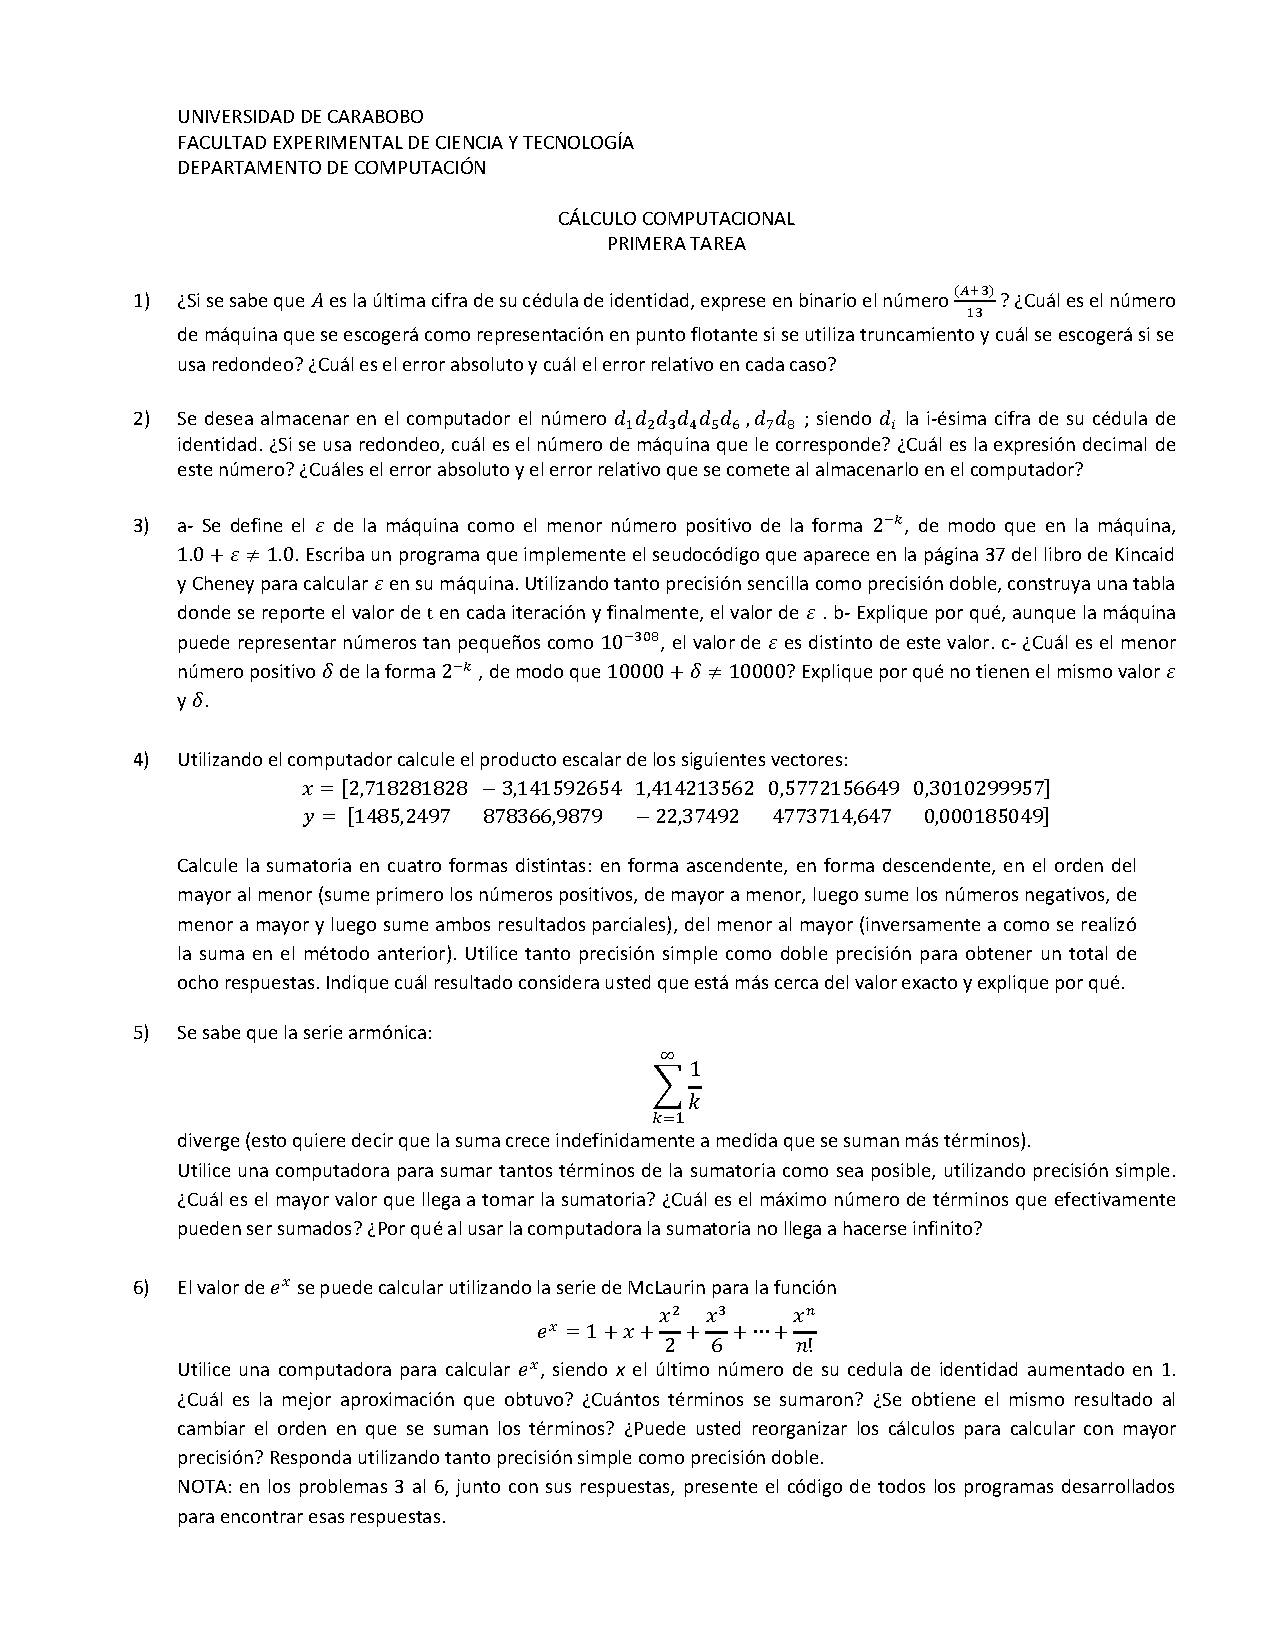
\includepdf[scale=0.8,pages=1,pagecommand=\subsection*{Enunciado Original}]{../Primera_tarea_Semestre_I_2016}

%%FIN CUERPO PRINCIPAl%%%%%%%%%%%%%%%%%%



% Codigo Fuente %%%%%%%%%%%%%%%%%%%%%%%%
%\newpage
%\begin{centering}
%	\section*{Código Fuente}
%\end{centering}

%\section*{repuesta3.c}
%\inputminted[
%frame=lines,
%framesep=2mm,
%baselinestretch=1.2,
%fontsize=\footnotesize,
%linenos
%]{c}{../Codigos/respuesta3.c}
%%%%%%%%%%%%%%%%%%%%%%%%%%%%%%%%%%%%%%%%%%%%%%%%%%%%%%

\end{document}
